\documentclass[11pt,a4paper]{article}
\usepackage[utf8]{inputenc}
\usepackage{amsmath}
\usepackage{amsfonts}
\usepackage{amssymb}
\usepackage{graphicx}
\usepackage{hyperref}
\usepackage{cite}
\usepackage{minted}
\usepackage{wrapfig}
\usepackage{hyperref}
\renewcommand{\baselinestretch}{1.5}
\renewcommand{\figurename}{Abbildung}
\renewcommand{\contentsname}{Inhalt}

\newcommand{\picturesource}[2]{\item {\figurename} \ref{#1}: \href{#2}{#2}}

\author{Clara Maier, Nico Fröhlich}
\title{Seminarkurs - Alan Turing}

\begin{document}
\maketitle
\newpage
\emph{Hiermit versichern wir, die vorliegende Arbeit selbstständig und nur unter Zuhilfenahme der angegeben Quellen und Hilfsmittel angefertigt zu haben. Aus den angegebenen Materialien entnommene Inhalte und Zitate sind als solche kenntlich gemacht. Wir erklären, dass wir zu diesem Thema nicht schon einmal eine solche Arbeit angefertigt habe.}
\newpage
\section{Vorwort}
Der Vater des Computer, die Person die wahrscheinlich den zweiten Weltkrieg um zwei Jahre verkürzte, was gibt es da noch zu sagen? Alan Turing eine der bekanntesten und einflussreichsten Mathematiker des letzten Jahrhunderts. Er beeinflusst nicht nur die Mathematik und heutige Informationstechnik, durch die Turingmaschine zum Beispiel, sondern auch die Philosophie, durch zum Beispiel den Turing Test. In seinem meist Zitierten Papier ging es sogar um Biologie. Am bekanntesten, nicht zuletzt durch den Film 'the imitation game', ist jedoch seine Beteiligung am zweiten Weltkrieg, durch die Entschlüsselung der Enigma der Nazis. Seine Arbeit im Bereich Computer Technik sowie in Ethik, Philosophie, sein Papier über Maschinen und Intelligenz sind mehr als nur Interessant. Sie sind weit mehr als das. Turing hat mit diesen Werken unsere heutiges Leben maßgeblich beeinflusst. In den Folgenden Kapiteln wird die tragische Geschichte rund um Alan Turing und ein paar seiner Zeitgenossen beleuchtet. Die Turing Maschine der Turing Test und seine Auswirkungen auf die Zukunft, sowie die Turing-Church-Hypothese werden in den Folgenden Abschnitten beleuchtet.
\tableofcontents
\newpage
\section{Historie}
Alan Mathison Turing wurde 1912, am 23 Juni in London geboren. Er starb am 7 Juni 1954 im Alter von 42 Jahren an seinem Wohnort in Wilmslow in Cheshire.
Seine Eltern Ethel und Julius Turing sind für seine Geburt  
\section{Enigma und Turing Bombe}
\label{enigma}
In diesem Abschnitt wird die Enigma und ihre Entschlüsselung thematisiert. Des weiteren wird auf die historischen Hintergründe eingegangen, auf ihre Funktionsweise sowie ihre Fehler.

\subsection{Enigma}
Die Enigma ist eine Verschlüsselungsmaschine, die im zweiten Weltkrieg von den Deutschen genutzt wurde um militärische Fernkommunikation zwischen ihren Truppen zu etablieren. Diese sollte ihnen mit unter einen entschiedenen Vorteil liefern. Dennoch hatte diese Verschlüsselung ein paar sehr große Probleme, die dazu führten, dass die Alliierten immer wieder sehr viele Informationen entschlüsseln konnten.\\
Hauptbestandteile der Enigma waren:
\begin{enumerate}
\item Eingabetastatur
\item Lichtanzeige
\item Steckbrett
\item Reflektor
\item drei oder vier Walzen
\end{enumerate}

\subsubsection{Eingabetastatur}
Eine zur Schreibmaschinen ähnliche Tastatur mit allen 26 Buchstaben des Alphabets, in die man die Nachricht eintippen konnte. Diese Tastatur war mit dem Steckbrett verknüpft.

\subsubsection{Lichtanzeige}
Eine Anzeige mit allen 26 Buchstaben des Alphabets, die einzeln beleuchtet werden und die verschlüsselte Nachricht anzeigen z.B ein H wird eingetippt und ein R wird beleuchtet.

\subsubsection{Steckbrett}
\label{sec:steck}
Das Steckbrett, welches hinten an der Enigma angebracht war, diente zur weiteren Verschlüsselung, da man hier bis zu 13 von 26 Buchstaben manuell miteinander verlinken konnte. Somit wurde z.B. ein eingegebenes A zu einem H und vice versa. Wenn kein Kabel eingesteckt wurde, dann wurde der Buchstabe einfach normal durch geschalltet. Meist wurden nur 10 umgesteckt, da sonst die Anzahl der Möglichkeiten wieder geringer wurden.

\subsubsection{Walzen}
\label{sec:rader}
\begin{wrapfigure}{r}{5cm}

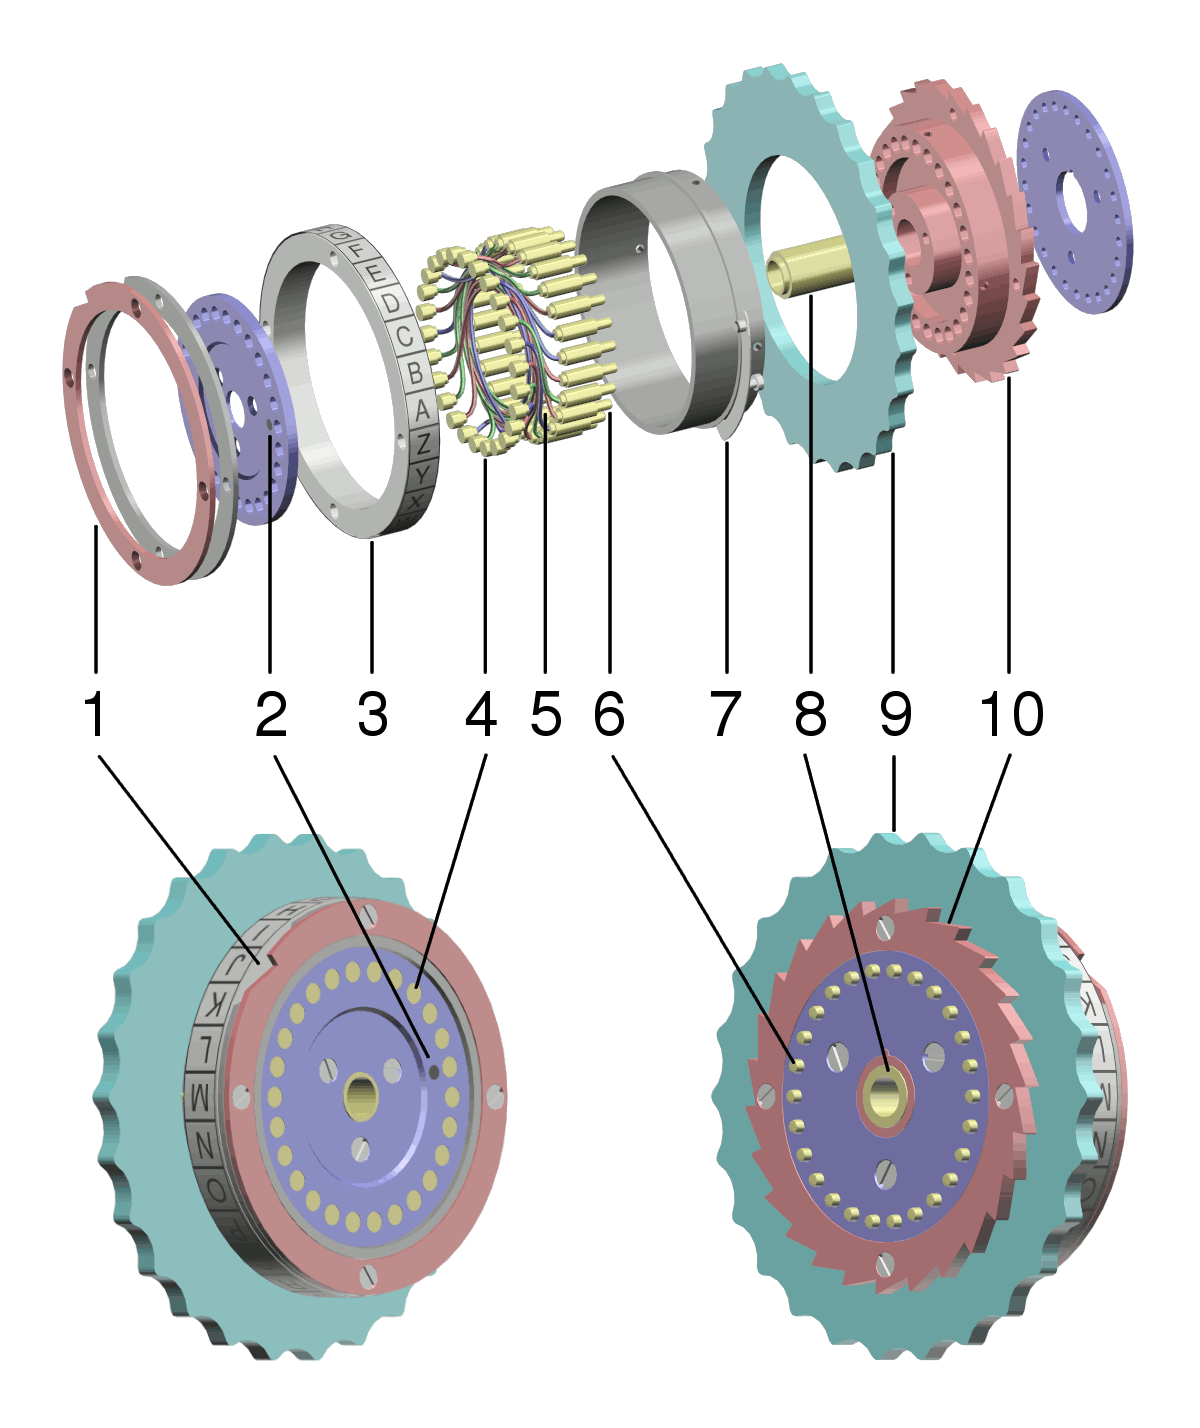
\includegraphics[scale=0.15]{Enigma_rotor_exploded_view.png}
\caption{Alan Turing}
\label{fig:rotorex}
\end{wrapfigure}
Die Walzen dienten zum weiteren Verschlüsseln der Nachrichten und jeder Walze hatte 26 Stufen für jeden Buchstaben des Alphabets. Wobei das Signal nun innerhalb der Walze durch neue Verkabelung auf einen anderen Buchstaben geleitet wurde (sog. rewiring). Das Signal wurde an die nächste Walze weiter geleitet, dort passiert das selbe nochmal. Es gab 8 verschiedene Arten von Walzen, diese besaßen pro Art immer eine andere Verkabelung innerhalb der Walzen. Walzen der gleichen Art hatten aber immer die selbe Verkabelung. Die erste Walze, welches die Eingabe passierte drehte sich bei jedem Tastendruck um einen Buchstaben weiter. Die nachfolgenden Walzen drehten sich immer dann um eines wenn sich das vorherige an seinem Überrollpunkt befindet. Dieser ist meist wenn sich die Walze einmal um sich selber gedreht hat, dass kann etwa bei M oder aber auch Z sein. Der Überrollpunkt konnte über eine Offset-Markierung an den Walzen eingestellt werden (sog. ring setting), so dass sich die Neuverkabelung um so viele Stellen wie eingestellt in eine Richtung weiter drehten. Diese wurden am Anfang jeder Nachricht einmal eingestellt. Am Anfang wurden diese Starteinstellungen über die Nachricht mitgeteilt, in dem man ein deutsches Wort mit 3 Buchstaben zweimal hintereinander gesendet hat. Was sich jedoch schnell als ziemlich schlechte Idee herausstellte und somit 1938 verboten wurde.

\subsubsection{Reflektor}
Der Reflektor schickte die Signale die von den Rollen kamen durch eine andere Leitung an den Rollen wieder zurück. Dieser konnte nie zum gleichen Buchstaben zurück senden sondern wurde wieder neu verkabelt.

\subsubsection{Beispiel}

\begin{figure}[H]
\centering
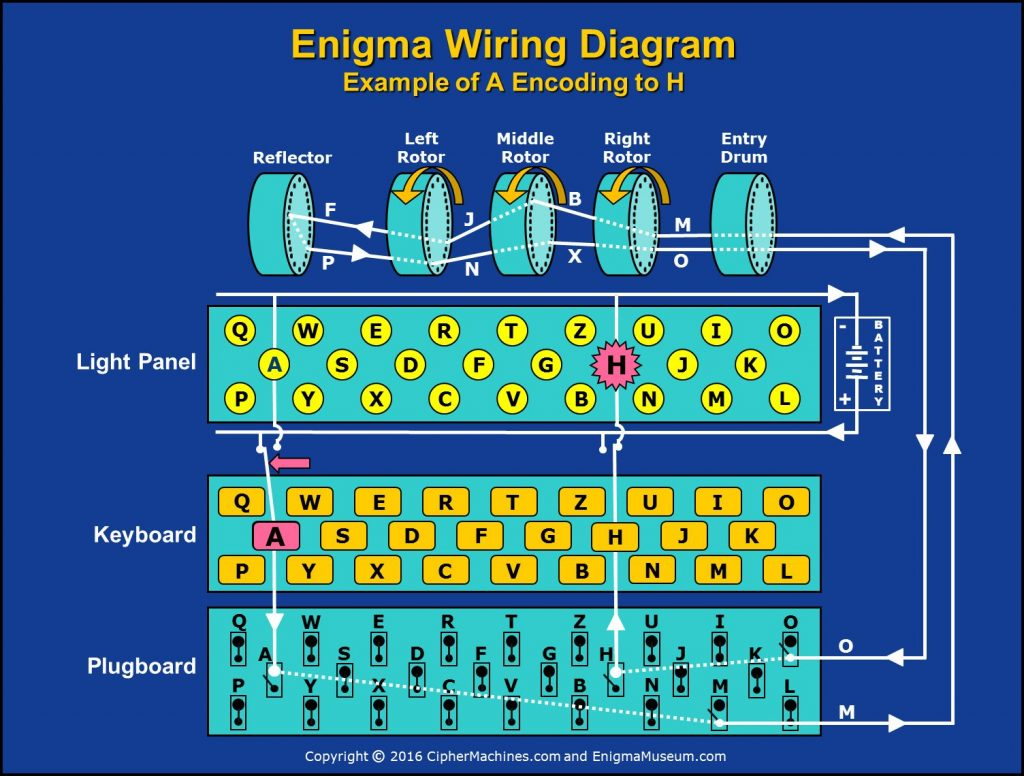
\includegraphics[scale=0.3]{Enigma_Maschine_Beispiel.jpg}
\caption{Beispiel Verkabelung}
\label{fig:enigma}
\end{figure}

Der eingegebene Buchstabe A geht erst einmal an das Steckbrett und ist hier mit dem Buchstaben M verbunden. Dieser wird dann an die Walzen weitergegeben, die den Buchstaben je nach Stellung verändern, hier von M zu B zu J und schließlich zu F. Anschließend wird der Buchstabe wieder zurück durch die Walzen geleitet und kommt in diesem Beispiel als O heraus und wird wieder an das Steckbrett weitergeleitet. Der Buchstabe O ist hier mit H verbunden und so wird am Ende H in der Anzeige beleuchtet, und somit wurde A zu H verschlüsselt.

\subsection{Historie}
Turing beschäftigte sich bereits vor Beginn des zweiten Weltkriegs mit den Enigma Maschinen. Diese waren jedoch von den Italienern und wesentlich simpler als die Enigma Maschinen, die später von den Deutschen eingesetzt wurden. Die erste Version der Enigma war frei verkäuflich und wurde eher privat genutzt da sie nicht viel Sicherheit bot. In dieser Version gab es lediglich 3 der in Sektion \ref{sec:rader} beschriebenen Räder, die in unterschiedlicher Reihenfolge eingesetzt werden konnten. Damit gab es lediglich $3! = 6$ Anordnungsmöglichkeiten. Zu dieser Zeit gab es außerdem kein, wie in Sektion \ref{sec:steck} aufgeführtes Steckbrett. Ein polnisches Verschlüsselungsteam unter der Leitung von Marian Rejewski legte den Grundstein und knackte die Verschlüsselungen der Enigma sehr schnell, dort wurden sie zum ersten mal mit Steckbrett Versionen konfrontiert. Diese knackten sie von Hand mit Hilfe von Lochpapieren. Deutschland wollte sich diese Verschlüsselungsmaschinen nun für militärische Zwecke zu nutzen machen, so entwickelten sie die nächste Version, die militärische Enigma. In dieser Version wurden zwei Walzen zur Auswahl hinzugefügt. Nun wurden also 3 aus 5 Walzen genommen und in unterschiedlichen Anordnungen in der Enigma kombiniert. Diese wurden nachher großflächig für die deutsche Luftwaffe und Armee eingesetzt. Doch der Marine war das nicht genug. Unter Admiral Karl Dönitz wurde eine Enigma speziell für die Marine entwickelt, bei der zu erst 3 aus 8 Walzen und später dann 4 aus 8 Walzen für die Verschlüsselung verwendet wurden. Zu allem Überfluss drehten sich die Räder 6 bis 8 zweimal an ihrem Überrollpunkt. Damit explodierten die möglichen Kombinationen fast exponentiell. Bei Ausbruch des Krieges wurde Turing zusammen mit Neuntausend anderen Spezialisten in den Bletchley Park geholt. Dieser Park wurde zu einer wahren Entschlüsselungsfabrik, in dem später mit Hilfe der \emph{Bombe}, 39 Tausend Enigma Nachrichten im Monat entschlüsselt wurden. Die sogenannte \emph{Bombe} war eine automatisierte Maschine zur Entschlüsselung der Enigma Nachrichten. Diese wurde ursprünglich von den Polen bis zur Invasion entwickelt. Durch die Invasion jedoch übergaben sie die von den Polen \emph{Bomba} genannte Maschine an die Briten. Dort verbesserten sie die Maschine weiter und bauten im Zuge des Krieges zwischen 60 und 100 verschiedene \emph{Bombes} in Großbritannien und noch einmal mindestens so viel in der USA. Dort halfen sie den Briten beim dechiffrieren per Unterseekabel. In Bletchley Park wurde der Platz sehr eng, deswegen wurden um das eigentliche Gebäude mehrere Hütten gebaut, die sogenannten \emph{Huts}. Schnell bekamen die \emph{Huts} spezielle Aufgaben. So war Hut 8, der Arbeitsplatz von Turing, mit der Entschlüsselung der sehr schweren Marine Enigma betraut. Die normalen Enigma Texte der Armee und der Luftwaffe wiederum, wurden in Hut 6 unter der Leitung von Gordon Welchman, ein weiterer berühmter Statistiker, bearbeitet.  \cite{enigmaproblem1} \cite{theessentialturing}

\subsection{Anzahl der Möglichkeiten}
Da die Turing Bombe größtenteils versucht hat den Code durch ausprobieren heraus zu finden, war das schier unmöglich auf Grund der Anzahl an Möglichkeiten. Dennoch konnte man die Anzahl an Möglichkeiten reduzieren (siehe nächstes Kapitel). Hier möchte ich einmal auf die Anzahl der Möglichkeiten bei einer normalen Enigma der Arme eingehen. Dadurch das man 3 aus 5 Rotoren auswählen musste ergibt sich $5 \cdot 4 \cdot 3 = 60$ Möglichkeiten (hier gilt ziehen ohne zurücklegen, da nie zwei Walzen der gleichen Art in der Enigma waren). Dazu kommen noch die Ringeinstellungen. Hier gab es für jede Walze eine Ringeinstellung mit je 26 Möglichkeiten bei 3 Walzen macht $26^3 = 17576$ Möglichkeiten oben drauf. Das schlimmste war jedoch das Steckbrett. Es gibt $!26$ Möglichkeiten Buchstaben mit einander zu kombinieren. Hier wurden jedoch immer nur 20 Buchstaben neu verbunden, somit bleiben 6 übrig also $!6$. Die Ordnung der Verbindungen ist uns egal sowie AB ist das gleiche als BA. Somit gibt es für das Steckbrett $\dfrac{!26}{2^{10}\cdot!6\cdot!10}$ das sind Rund $1.5 \cdot 10^{13}$ Möglichkeiten. Wenn man alle Möglichkeiten zusammen rechnet kommt man auf Rund $1.6 \cdot 10^{20}$  Möglichkeiten\cite{emach}

\subsection{Schwachstellen}
Die Enigma hatte einige Schwachstellen, die im ersten Moment vielleicht nicht als solche erscheinen. Dazu gehörte einmal, dass der Reflektor die Signale nie auf den gleichen Buchstaben zurück leiten konnte. Dadurch konnte man versuchen bekannte Wörter wie zum Beispiel "Wetterbericht" unter den verschlüsselten Text zu halten. Wenn einer der Buchstaben in dem Wort mit dem verschlüsselten Text an der Stelle übereinstimmte, dann konnte es sich nicht um das Wort handeln. Ziel der Entschlüsselung war es heraus zu finden mit welchen der Räder und mit welchen Walzeneinstellungen sie die \emph{Bombe} bestücken mussten. Diese sollte dann automatisch die Nachrichten entschlüsseln. Des weiteren war bei den Rollen 6 bis 8 der Marine das zweite Überrollen ein Indikator dafür, dass eine solche Walze eingesetzt wurde. Dies konnte die Möglichkeiten sehr einschränken. Das oben genannte Problem mit dem doppelt senden eines deutschen Wortes mit 3 Buchstaben hat natürlich dafür gesorgt, dass hier über die Wahrscheinlichkeiten in der Sprache es sehr einfach war die Ringeinstellung zu erraten. Mit Hilfe des oben genannten Reflektor Problems minimierte es natürlich weiter die Möglichkeiten. Dieses Problem bemerkten die Deutschen und verbaten diese Übersendung von Ringeinstellungen. Des weiteren halfen gestohlene Codebücher und Insiderinformationen beim Entschlüsseln. Dazu kam, dass die Deutschen jeden Morgen  um Punkt 6 Uhr ihren Wetterbericht sendeten, denn dieser begann mit dem Wort \emph{Wetterbricht} und endete mit \emph{Heil Hitler}. \cite{enigmaflaw} \cite{enigmaproblem1}
\section{Turing Maschine}
Die Turingmaschine wurde 1936 von Alan Turing entwickelt und ist rein theoretisch, denn eine Maschine exakt wie es Turing beschreibt wurde niemals gebaut, da dies auch nicht sinnvoll wäre. Turing entwickelte diese Theorie aufrund des Entscheidungsproblem von David Hilber und Wilhelm Ackermann \cite{theessentialturing}. Die Turing Maschine ist die heutige Grundlage vieler Programmiersprachen, wie Java, C++ oder Phyton. Diese Programmiersprachen werden auch als Turing complete bezeichnet, was so viel heißt wie dass die Turing Maschine diese theoretischer weiße emulieren kann.

\subsection{Funktion} 
Die Turing Maschine beinhaltet lediglich zwei Bauteile.
\begin{enumerate}
\item  Ein unendlich langes Band, dass in eine Kette von horizontalen Kästchen eingteilt ist. Jedes dieser Kästchen kann entweder eine 0,eine 1 oder auch nichts beinhalten. Zudem kann das Band nach rechts und nach links verschoben werden.
\item Ein Kasten auch "Heap" genannt, der die Zahlen auf dem Band einlesen,löschen und ändern kann.
\end{enumerate}
 


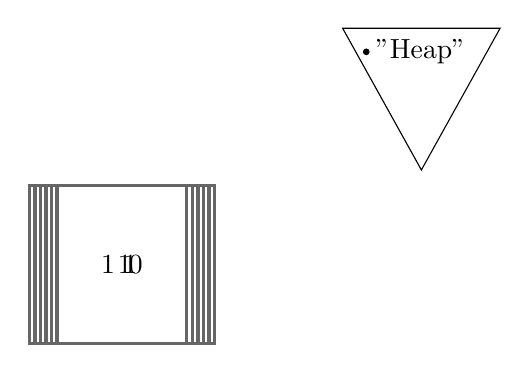
\begin{tikzpicture}[
squarednode/.style={rectangle, draw=black!60, very thick, minimum size=20mm}
]
%Nodes
\node[squarednode][right=0] {1};
\node[squarednode][right=2]{ };
\node[squarednode][right=4]{ };
\node[squarednode][right=6]{1};
\node[squarednode][right=8]{1};
\node[squarednode][right=10]{0};
 
%Lines
\draw[black](4,3) -- (5,1.2) -- (6,3) -- cycle;
\filldraw[black] (4.3,2.7) circle (1pt) node[anchor=west] {"Heap"}; %??????


\end{tikzpicture}



\subsection{Beispiel} Zur besseren Vorstellung, erkläre ich das Ganze nochmal an einem Beispiel. Nehmen wir mal an wir wollen, dass die Turing Maschine für uns unendlich Hochzählt. So kann man dies mit nur zwei einfachen Befehlen ausführen. 

\begin{itemize}
\item Befehl 1 = Bei einer 1, ändere diese in eine 0 und gehe nach links 
\item Befehl 2 = Bei einer 0 oder einer Lücke, ändere diese in eine 1 und gehe zum letzten Bit der Zahl 
\end{itemize}

Die Befehle für die Turing Maschine kann man sich also heute wie die Programme auf unseren Computern vorstellen.
\section{Turingtest}
\label{turingtest}
In diesem Abschnitt geht es um Turings Ausflug in die Philosophie und sein Werk "Computing Machinery and Intelligence". Dabei wird die Frage betrachtet ob Maschinen denken können und wie man eine Maschine von einen Menschen unterscheiden kann. Sowie heutige Anwendungen und Auswirkungen auf Kunst und Gesellschaft.
\subsection{The Imitation Game}
Turing stellt eine bessere Frage in den Raum, als die Frage "Können Maschinen Denken?". Um die Frage allerdings stellen zu können muss ich das "Imitation Game" einführen. Das Spiel funktioniert wie folgt. Lass A ein Mann sein, B eine Frau und C einen Detektiv. Der Detektiv (C) will also heraus finden wer welches Geschlecht hat, ohne dabei die Sprache zu hören oder die Person zu sehen. Um diesen Zustand zu gewährleisten gehen wir davon aus, dass der Detektiv in einem anderen Raum ist wie A und B, die einzige Kommunikation die besteht ist also textbasiert. Also versucht C Fragen zu verwenden, um mit Hilfe der Antworten beider Personen zu bestimmen, welche weiblich und welcher männlich ist. Dies wendet Turing nun auf Maschinen an, dabei beschränkt er sich auf Digitalcomputer. Es wird versucht auf äußerliche Fragen zu verzichten, da dies zu keinem eindeutigen Ergebnis führen würde. Die Maschine könnte ganz einfach ein eigenes fingiertes Aussehen annehmen und die Person kennt ihres, daher ist es schwierig anhand der Antworten eindeutig zu unterscheiden. Deshalb versucht C logische Fragen zu verwenden um heraus zu finden ob es sich um eine reale Person handelt. Beispiel: Subtrahiere 56 von 18934.\cite{computing} Dieses Spiel wird nun nicht nur dazu genutzt eine Maschine von einem Menschen zu unterscheiden, sondern es wird implizit die Frage gestellt ob eine Maschine denken kann. Wenn man ihre Antworten nämlich nicht mehr voneinander unterscheiden kann, muss man sich Gedanken darüber mache,  ob wir dann nicht intelligentes Leben geschaffen haben könnten und wie wir dieses dann behandeln.
\subsection{Chinese room problem}
Eine der berühmtesten Probleme des Turing Tests ist das chinese room problem. Dieses Problem stellt in Frage, ob man mit dem Turingtest wirklich die Intelligenz eines Lebewesens feststellen kann. Dabei wird eine weitere Situation angenommen. Nehmen wir also an zwei Personen sitzen sich gegenüber in einem Raum. Die eine Person ist ein Chinese die andere Person ein Deutscher. Auf dem Tisch liegt nun ein Deutsch-Chinesisch Wörterbuch. Die beiden Personen versuchen miteinander zu kommunizieren. Dazu nutzt der Deutsche ein Wörterbuch. Nun stellt sich die Frage, wenn der Deutsche nun seinen Satz auf Chinesisch übersetzt, ob er wirklich weiß was er sagt. Übertragen auf eine Maschine stellt sich nun ebenfalls die Frage, kann die Maschine wirklich wissen was sie tut und diese Aktionen auch selber hinterfragen. Darüber hinaus stellt sich die Frage wie intelligent Maschinen wirklich werden können.
\subsection{Anwendungen in der Moderne}
Hier folgt eine kurze Beleuchtung des heutigen Einsatzfeldes des Turing Tests. Dieser wird in der Internetsicherheit sehr oft verwendet um automatisierte Anfragen zu filtern. Als Beispiel wird hier exemplarisch ReCaptcha von Google beleuchtet. Es gibt aber genug andere sogenannte Captcha Methoden. Diese geben eine Art von Frage an, hierbei ist die Kommunikation allerdings nicht nur wie im Turing Test, auf textbasierte Kommunikation beschränkt. Im Gegenteil, hier werden sogar bewusst Bilder eingesetzt, damit der zu testende Computer beziehungsweise die Person die den Computer bedient, eine Frage zu diesen Bildern beantworten muss. Dabei sind die Antworten auf die eigentliche Frage nicht einmal so wichtig wie es einem im ersten Moment erscheint. Die Ironie, und eine weitere Abweichung ist dabei, dass man hier gegen ein neuronales Netzwerk "spielt". Dieses muss anhand der vorliegenden Informationen bestimmen, ob die Anfrage von einem Mensch stammt oder ob es sich dabei nur um eine automatisch generierte Anfrage handelt. Wie genau dieses Netzwerk entscheidet weiß wahrscheinlich nicht mal Google. Wichtig ist aber welche Daten dem Netzwerk dabei zur Verfügung gestellt werden, um seine Entscheidung zu treffen. Für weitere Informationen verweise ich hier auf einen Blog-Eintrag\cite{captcha}. Zu den auszuwertenden Daten gehören unter anderem die Mausbewegungen sowie die gesendeten Daten des Browsers (z.B. User-Agent, IP, Cookies).
\subsection{Auswirkungen auf Kunst und Gesellschaft}
Diese grundsätzlichen Gedanken und die Frage, ob Maschinen überhaupt denken können hat weitreichende Auswirkung auf die Moderne Kunst, darunter vor allem Computerspiele. Sehr gute Beispiele sind, das gleichnamige Spiel "The Turing Test" oder auch "The Talos Principle" in denen der Turing Test sehr häufig vorkommt. Es ist wichtig hier darauf aufmerksam zu machen, dass das Imitation Game heute noch für sehr viel Kopfzerbrechen unter den Wissenschaftlern, Philosophen so
wie in der gesamten Gesellschaft auslöst. Wir werden bald an den Zeitpunkt kommen wo es wichtig sein wird, sich mit dieser Frage auseinander zu setzen. Weiterführend dazu siehe The future of the mind: Exploring machine consciousness von Dr. Susan Schneider\cite{explorecons}



\section*{Bildquellen}
{\renewcommand\labelitemi{}
\begin{itemize}
\picturesource{fig:turing}{https://blog.sciencemuseum.org.uk/wp-content/uploads/2013/12/Alan-Turing-29-March-1951-picture-credit-NPL-Archive-Science-Museum1.jpg}
\picturesource{fig:enigmaset}{https://d1e4pidl3fu268.cloudfront.net/10fd7805-c5e4-
42ac-8f67-bc7d0a42e6d0/enigma\textunderscore machine.crop\textunderscore 720x540\textunderscore 68\%2C0.preview.jpg}
\picturesource{fig:rotorex}{https://de.wikipedia.org/wiki/Enigma-Walzen\# /media/Datei:Enigma\textunderscore rotor\textunderscore exploded\textunderscore view.png}
\picturesource{fig:enigma}{http://enigmamuseum.com/wp-content/uploads/2016/12/WiringDiagram-1024x776.jpg}
\end{itemize}
}

\bibliography{main}
\bibliographystyle{ieeetr}

\end{document}
